\subsection*{Модель роста R\&D}
\addcontentsline{toc}{subsection}{Модель роста R\&D}

\textbf{Задание:}\\
Провести численный и качественный анализ модели роста R\&D.\\

\textbf{Решение:}\\
\textit{Качественный анализ:}\\
$A$ -- знания в рассматриваемой экономике\\
$L$ -- общий объём труда\\
$K$ -- капитал\\
$Y$ -- агрегированный выпуск благ

\begin{align*}
& Y = [(1 - a_K)K]^\alpha [A (1 - a_L)L]^{1-\alpha}\\
& \dot{A} = B(a_K K)^\beta (a_L L)^\gamma A^\theta\\
& \dot{K} = sY - \delta K\\
& \dfrac{\dot{L}}{L} = n
\end{align*}

Ограничения на параметры: $B > 0$, $\beta \geq 0$, $\gamma \geq 0$, $0 < s < 1$, $n \geq 0$, $0 < \alpha < 1$.\\

Приведём данную модель к относительным показателям.

\[y = \dfrac{Y}{L} \]
\[k = \dfrac{K}{L} \]
\[a = \dfrac{A}{L} \]

\[\dot{k} = \left(\dfrac{K}{L}\right)' = \dfrac{\dot{K}L - K\dot{L}}{L^2} = \dfrac{\dot{K}}{L} - \dfrac{K}{L} \dfrac{\dot{L}}{L} = \dfrac{sY - \delta K}{L} - kn = sy - \delta k - kn = sy - (n + \delta)k \]

\[Y = \left[(1 - a_K) \dfrac{K}{L} \times L \right]^\alpha \left[\dfrac{A}{L} \times L (1 - a_L) L \right]^{1 - \alpha} = ([(1 - a_K) k \times L]^\alpha [a \times L(1 - a_L)L]^{1-\alpha}) = \]
\[ = (1 - a_K)^\alpha k^\alpha (1 - a_L)^{1-\alpha} a^{1-\alpha} L^{2 - \alpha} \]
\[y = (1 - a_K)^\alpha k^\alpha (1 - a_L)^{1 - \alpha} a^{1 - \alpha} L^{1 - \alpha} \]

\newpage

\[\dot{a} = \left(\dfrac{A}{L}\right)' = \dfrac{\dot{A}L - A\dot{L}}{L^2} = \dfrac{\dot{A}}{L} - \dfrac{A}{L} \dfrac{\dot{L}}{L} = \dfrac{B(a_K K)^\beta (a_L L)^\gamma A^\theta}{L} - an = \]
\[ = \dfrac{B(a_K \frac{K}{L}L)^\beta (a_L L)^\gamma (\frac{A}{L} L)^\theta}{L} - an = B(a_K k L)^\beta (a_L L)^\gamma a^\theta L^{\theta - 1} - an \]

\[ \dot{k} = sy - \delta k - kn = sy - (n + \delta) k = s ((1 - a_K)^\alpha k^\alpha (1 - a_L)^{1 - \alpha} a^{1 - \alpha} L^{2 - \alpha}) - \delta k - k n \]

\[ \dot{a} = B(a_K k L)^\beta (a_L L)^\gamma a^\theta L^{\theta - 1} - an \]

\textit{Численный анализ:}\\
В соответствии с формулами, данная модель была реализована в среде моделирования AnyLogic. (Рисунок \ref{fig:randd1})
\begin{figure}[h]
	\centering 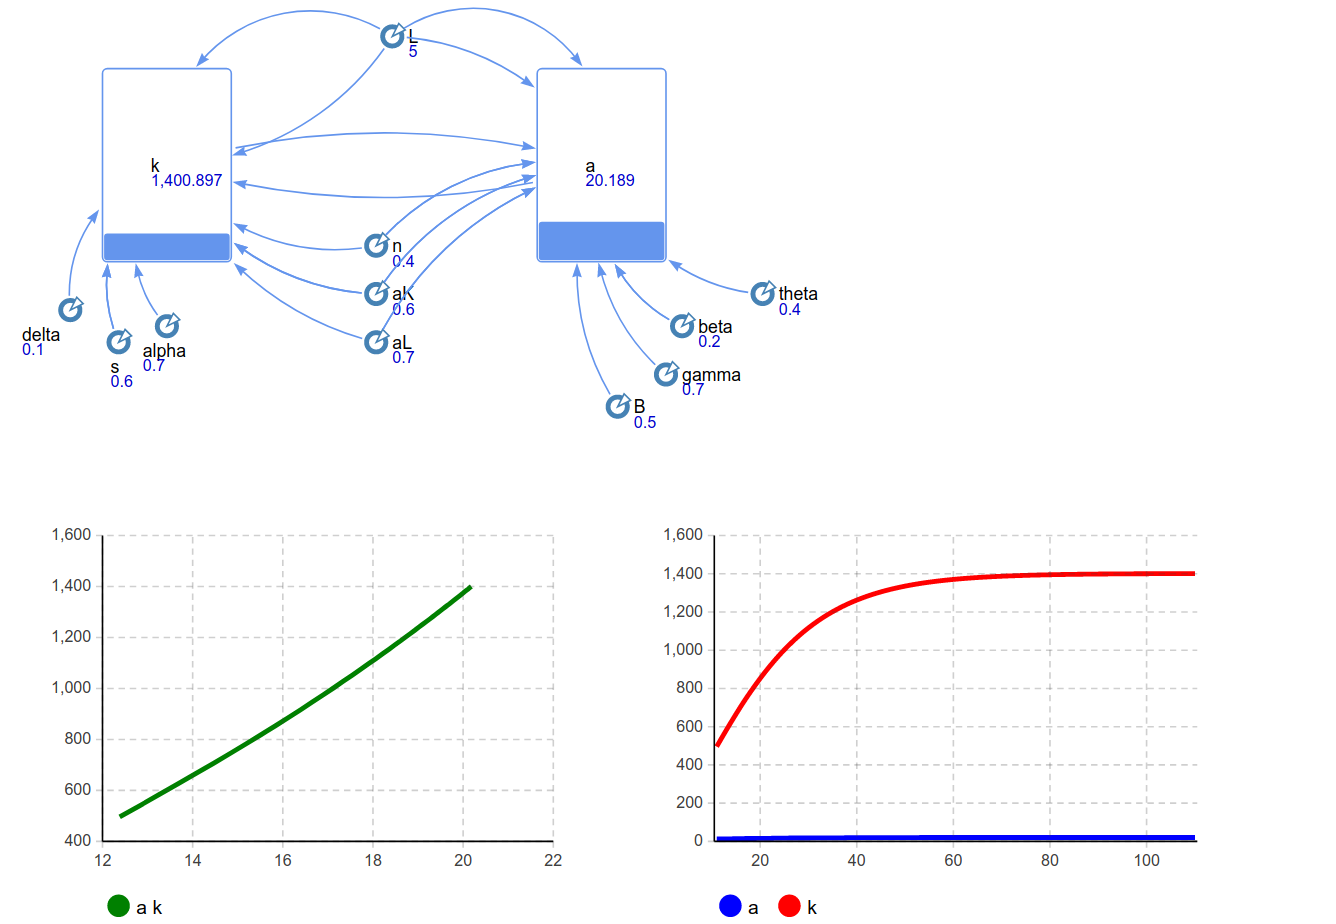
\includegraphics[scale=0.3]{randd1}
	\caption{Результаты построения модели R\&D в AnyLogic}
	\label{fig:randd1}
\end{figure}

В ходе симуляции было получено состояние равновесия -- устойчивый узел.\\

Таким образом, была построена и проанализирована модель роста R\&D.\\